\documentclass[tikz]{standalone}
\usepackage{amsmath}
\usepackage{amssymb}
\begin{document}

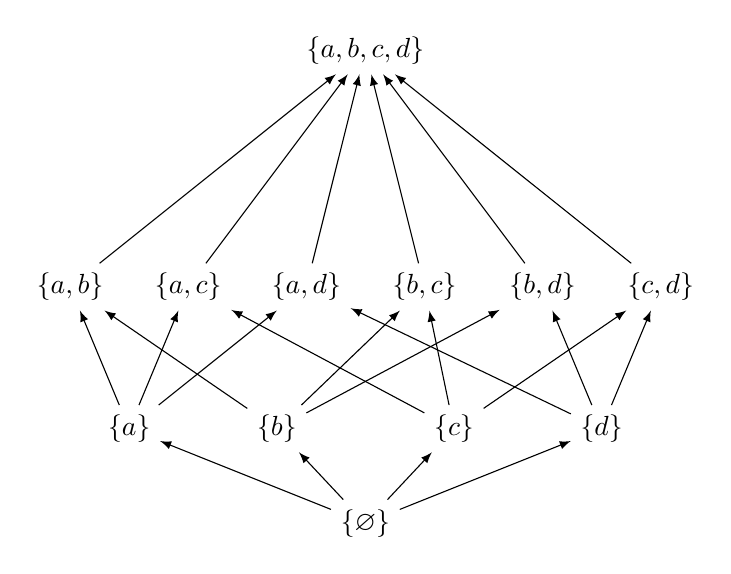
\begin{tikzpicture}[scale=1.5, >=latex,->]

	% === NODES === (((
	\node (0) at (-0.5,0) {\(\{\varnothing\}\)};

	\node (a) at (-2.5,0.8) {\(\{a\}\)};
	\node (b) at (-1.25,0.8) {\(\{b\}\)};
	\node (c) at (0.25,0.8) {\(\{c\}\)};
	\node (d) at (1.5,0.8) {\(\{d\}\)};

	\node (ab) at (-3,2) {\(\{a,b\}\)};
	\node (ac) at (-2,2) {\(\{a,c\}\)};
	\node (ad) at (-1,2) {\(\{a,d\}\)};
	\node (bc) at (0,2) {\(\{b,c\}\)};
	\node (bd) at (1,2) {\(\{b,d\}\)};
	\node (cd) at (2,2) {\(\{c,d\}\)};

	\node (abcd) at (-0.5,4) {\(\{a,b,c,d\}\)};
	% \node () at (<++>) {<++>};
	% )))

	% === LINES === (((
	\draw (0) -- (a);
	\draw (0) -- (b);
	\draw (0) -- (c);
	\draw (0) -- (d);

	\draw (a) -- (ab);
	\draw (a) -- (ac);
	\draw (a) -- (ad);

	\draw (b) -- (ab);
	\draw (b) -- (bc);
	\draw (b) -- (bd);

	\draw (c) -- (ac);
	\draw (c) -- (bc);
	\draw (c) -- (cd);

	\draw (d) -- (ad);
	\draw (d) -- (bd);
	\draw (d) -- (cd);

	\draw (ab) -- (abcd);
	\draw (ac) -- (abcd);
	\draw (ad) -- (abcd);
	\draw (bc) -- (abcd);
	\draw (bd) -- (abcd);
	\draw (cd) -- (abcd);
	% )))

\end{tikzpicture}

\end{document}
